% A workaround to allow relative paths in included subfiles
% that are to be compiled separately
% See https://tex.stackexchange.com/questions/153312/subfiles-inside-a-subfile-using-relative-paths
\providecommand{\main}{..}
\documentclass[\main/thesis.tex]{subfiles}

\begin{document}

\chapter{Introduction}

Current estimates suggest that human knowledge is doubling every 12 hours. A significant portion
of that knowledge is often stored in a format that is readable by humans. However, as humans come 
to rely more and more on computes and their ability to interpret and understand human knowledge, so
does the need for storing human knowledge in a format that is digestible by computers. This is where 
knowledge graphs come in. Knowledge graphs provide a way to represent and store knowledge in a 
graph-like structure where nodes represent entities and edges represent relationships between
entities. A prime example of a knowledge graph is the Google Knowledge Graph that is used 
by google power their search engine. 


Generally speaking, knowledge graphs are generated by painstaking manual human effort. 
This has changed with the advent of Large Language Models such as GPT2-XL that can now be used to
augment currently existing knowledge graphs\cite{west_symbolic_2021}. This not only 
reduces the cost of creating a knowledge graph but also allows for much faster creation 
of knowledge graphs which in turn can then be used to tune downstream models for better 
performance\cite{noauthor_kelm_2021}


\section{Knowledge Graphs}\label{sec:knowledgeGraphs}

There are multiple definitions of knowledge graphs. The most widely known one comes from Google's 
popularization of the word in 2012\cite{noauthor_introducing_2012} where the authors imply 
that the knowledge that Google contains is accessible via the Google knowledge graph. On the 
flip side, authors describe knowledge graphs as RDF graphs (a set of RDF triples)\cite{farber_linked_2017}. 
For our purposes, we will describe knowledge graphs as a set of RDF triples that contain 
a subject, a property and an object. Some example RDF triples are show in Figure\ref{fig:kg_fig}.

\begin{figure}
    \centering
    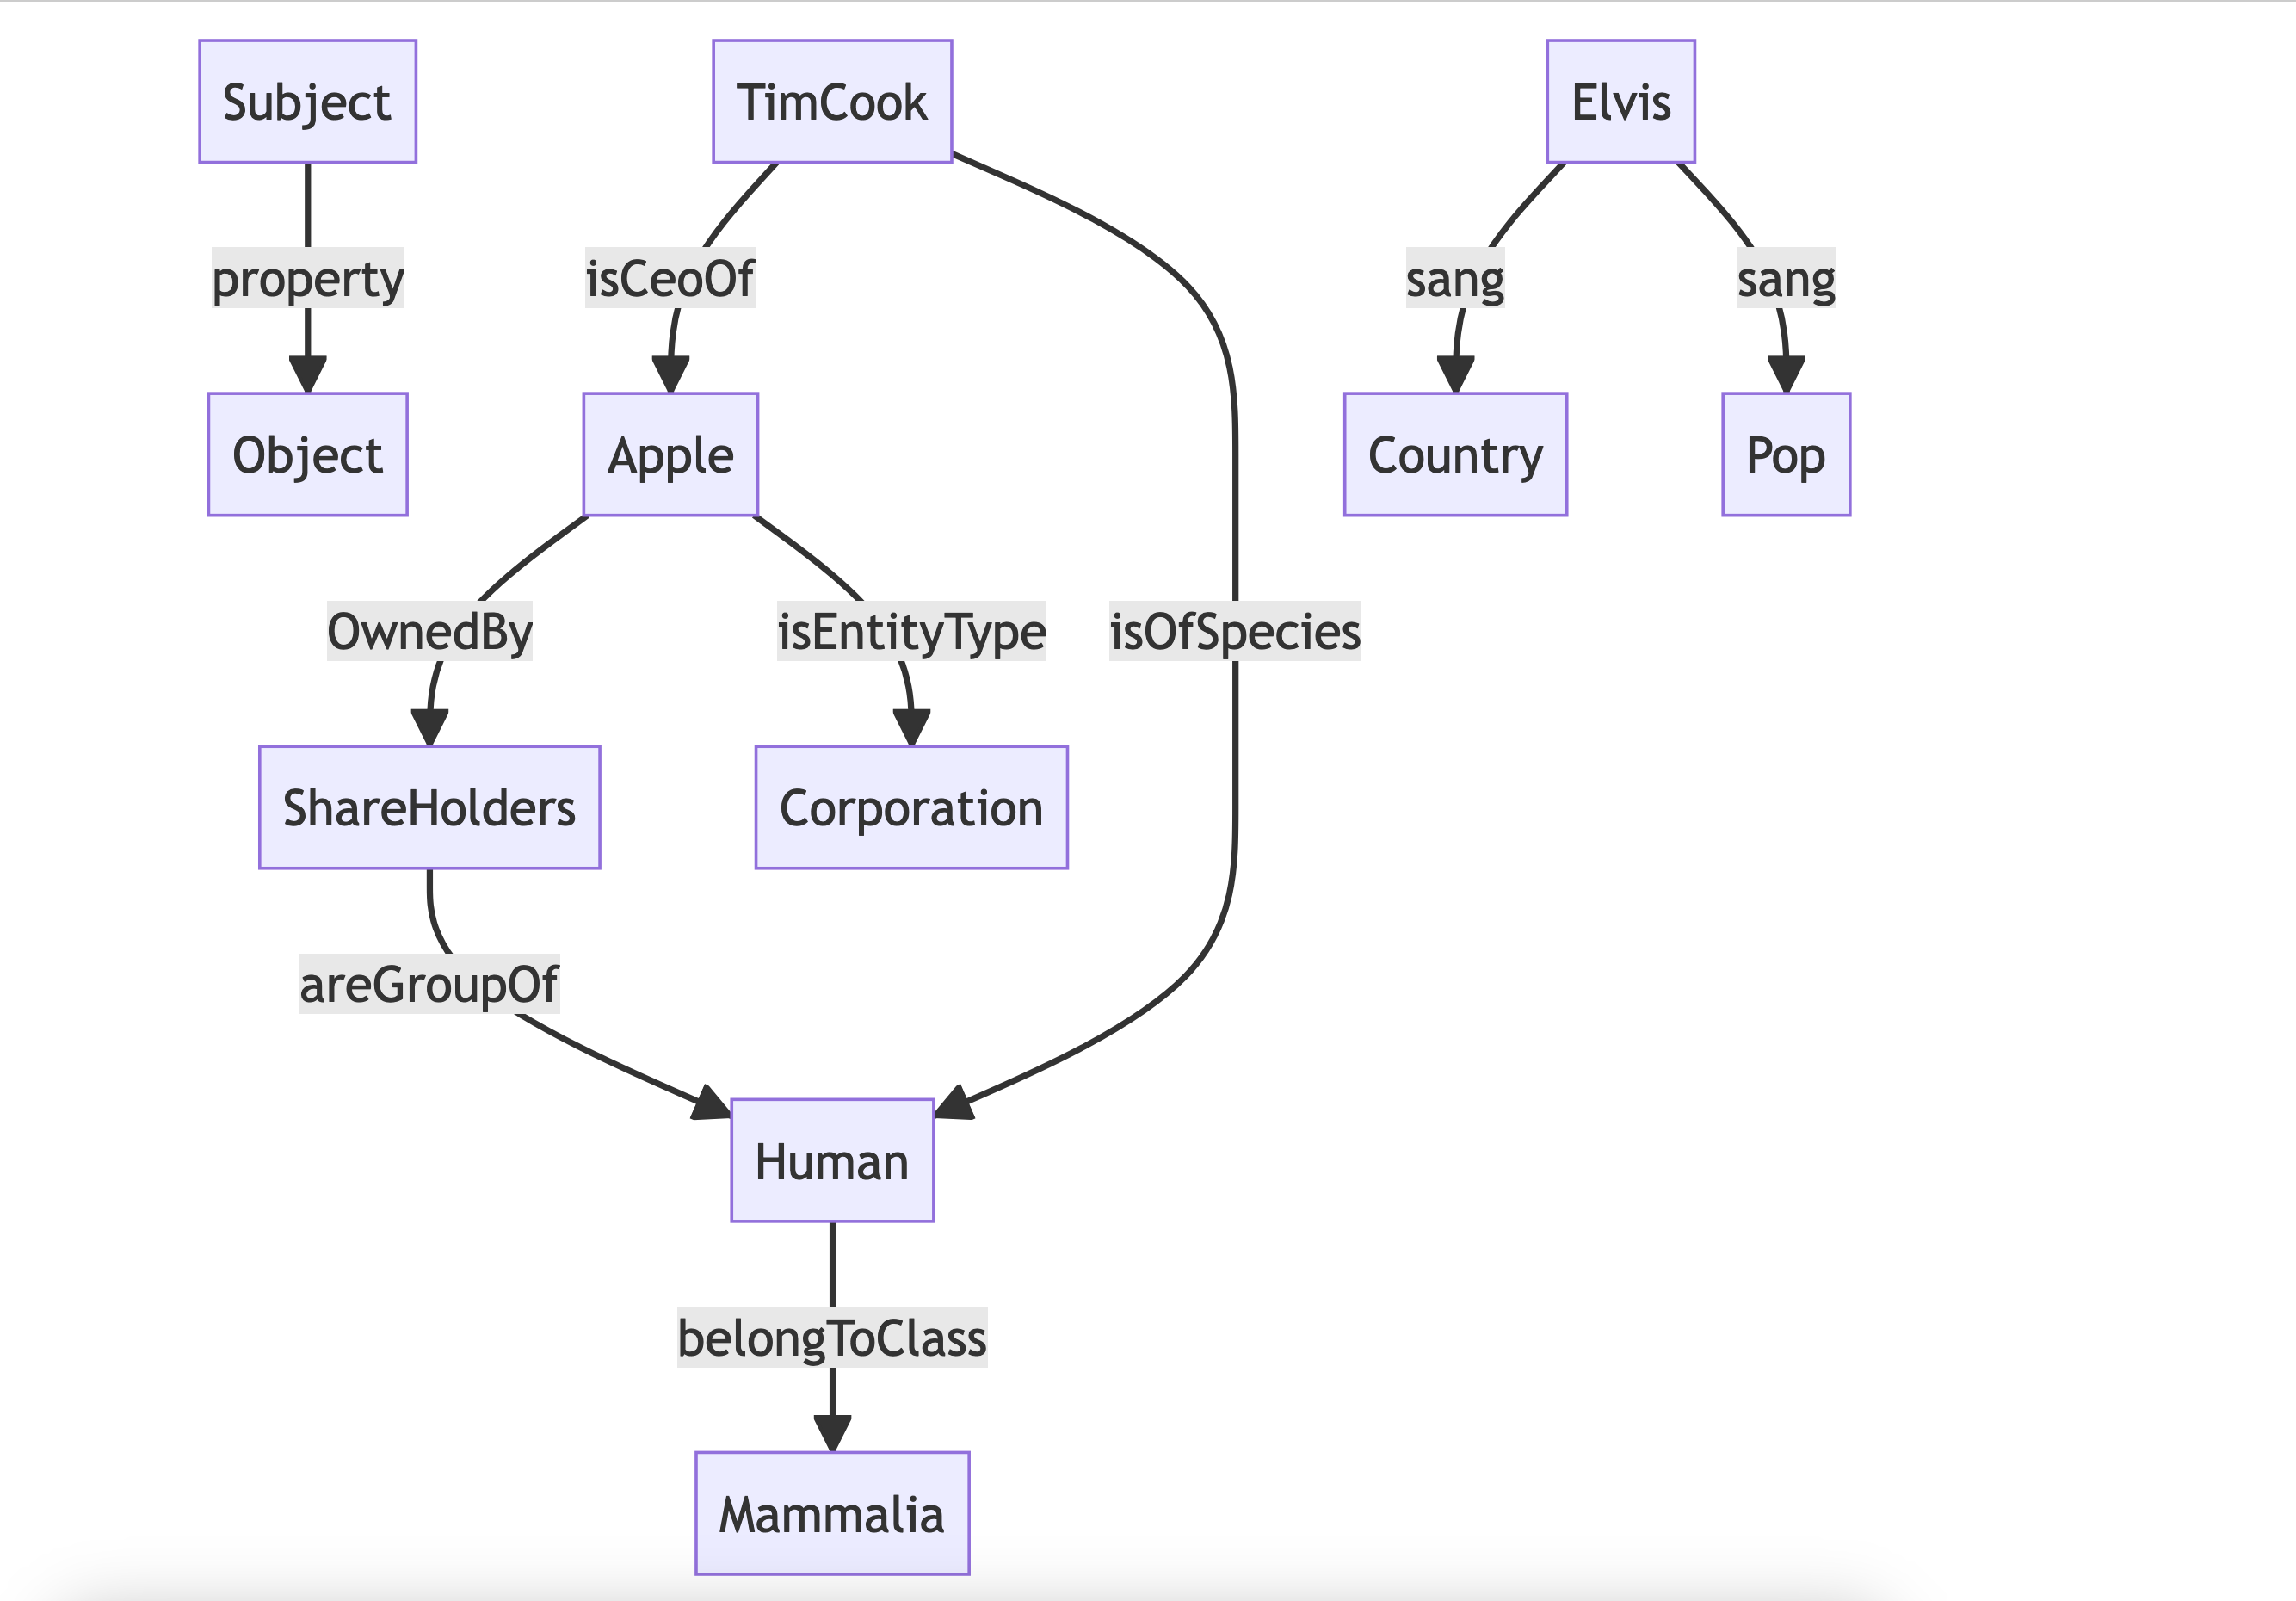
\includegraphics[keepaspectratio=true, width=0.9\textwidth]{\main/img/kg}
    \caption[Example RDF Triples] {Example RDF Triples}
    \label{fig:kg_fig}
    % Put the label *after* the caption, but inside the float
\end{figure}

There are several different types of knowledge graphs that exist today. A summary of some of 
most widely used is available below: 

\begin{enumerate}
    \item \textbf{Domain Specific Knowledge Graphs:} These knowledge graphs are created for a
    specific domain. An example of this would be a knowledge graph created for medical information. 
    \item \textbf{Semantic Web Knowledge Graphs:} These knowledge graphs are created by
    extracting information from the semantic web and adhere to the RDF and OWL standards.
    \item \textbf{Enterprise Knowledge Graphs:} These knowledge graphs are used to connect 
    and collate information from different sources within an enterprise allowing for better 
    search, recommendations and analytics.
\end{enumerate}

\section{Commmon Sense Knowledge Graphs}\label{sec:commonsenseKnowledgeGraphs}

The knowledge graph relevant to this project is the Commonsense Knowledge Graph (CSKG). 
As the name suggests, CSKGs aim to store and represent common sense knowledge as seen 
from a human's perspective. This can include a wide variety of concepts that range from
the simple such as "A person can be a parent of another person" to the more complex such as
"A person can be a parent of another person only if the first person is older than the second".
All of this these concepts help humans make sense of the world around them and are 
often taken for granted. However, for a computer to be able to make sense of the world
around it, it needs to be able to understand these concepts. This is where CSKGs come in.

Some widely known CSKGs are ConceptNet \cite{speer2018conceptnet} and 
ATOMIC \cite{sap_atomic_2018}. 
The former is a knowledge graph that contains over 34 million commonsense knowledge triples
that are of the form (subject, relation, object). It contains a vast array of information 
that has been used for a variety of Natural Language Processing tasks. 

The latter is a freely available knowledge graph that contains over 877k unique commonsense 
knowledge triples. The triples are of the form (subject, relation, object) where the 
relation is one of 14 different relations (e.g.) xNeed, xIntent, xAttr etc. 
This knowledge graph focuses on inferentail knowledge over taxanomic knowledge.


Commonsense knowledge plays a crucial role today in many machine learning applications including
natural language processing and computer vision. Commonsense is often provided via a number 
of sources dependening on the application. In order to provide a common source that can play
multiple roles, CommonSense Knowledge Graphs (CSKGs) were born \cite{ilievski_cskg_2021}.


\section{Large Language Models}\label{sec:largeLanguageModel}

Language models, in essense, are probablity distributions over sequences of words \cite{jurafsky_speech_2009}. 
They are used for a variety of purposes that range from the simple such as tab completion to 
sophisticated text generation and reviewing human written translations. 

Large language models are often based on a deep learning architecture such as a transformer
or a recurrent neural network. The models are trained on a large corpus of text 
(in the billions of documents) and require extensive computing resources to train and 
do inference with. The aim of the training process is to capture a generalized 
representation of the language that can then be used for a variety of tasks. 

With the advent of larger and more sophisticated language models such as GPT-3\cite{brown_language_2020}, the scope
of usefuless for language models has expanded significantly. One such use is in the 
augmentation of currently existing commonsense knowledge graphs \cite{west_symbolic_2021}.
This kind of usage requires that large language models (LLMs) such as GPT-2 be trained on the task
of knowledge generation. As per \citeauthor{west_symbolic_2021}, language models fail to express common 
sense knowledge when prompted in a zero-shot manner. As such, the authors converted the models
to COMET-DISTIL models by training them on a knowledge graph. We suspect, such training, while providing 
additional capabilities for knowledge graph generation, reduces other language modelling capabilities
of the trained model. 

\section{Transfomers}\label{sec:transformers}
In 2017, Vaswani et al. introduced the Transformer architecture \cite{vaswani2017attention}. 
This led to one of the widest adoptions of a single architecture in the field of Natural Language
Processing. The Transformer architecture is based on the concept of self-attention. 
Self-attention enables a model to learn contextual relationships between words in a sentence.
It does so by computing a weighted sum of the words in a sentence. The weights are computed
based on the similarity between the words. 

This architecture is being used in the model of interest for this project. It is also 
the most successful architecture for language modelling to date as evidenced in the form
of BERT, GPT-3 and other models.

\end{document}